\documentclass[border=10pt]{standalone}

\usepackage{tikz}
\usepackage{tikzsymbols}
\usetikzlibrary{calc,patterns,shapes.geometric}

\def\centerarc[#1](#2)(#3:#4:#5){\draw[#1] ($(#2)+({#5*cos(#3)},{#5*sin(#3)})$) arc (#3:#4:#5);}

\begin{document}
	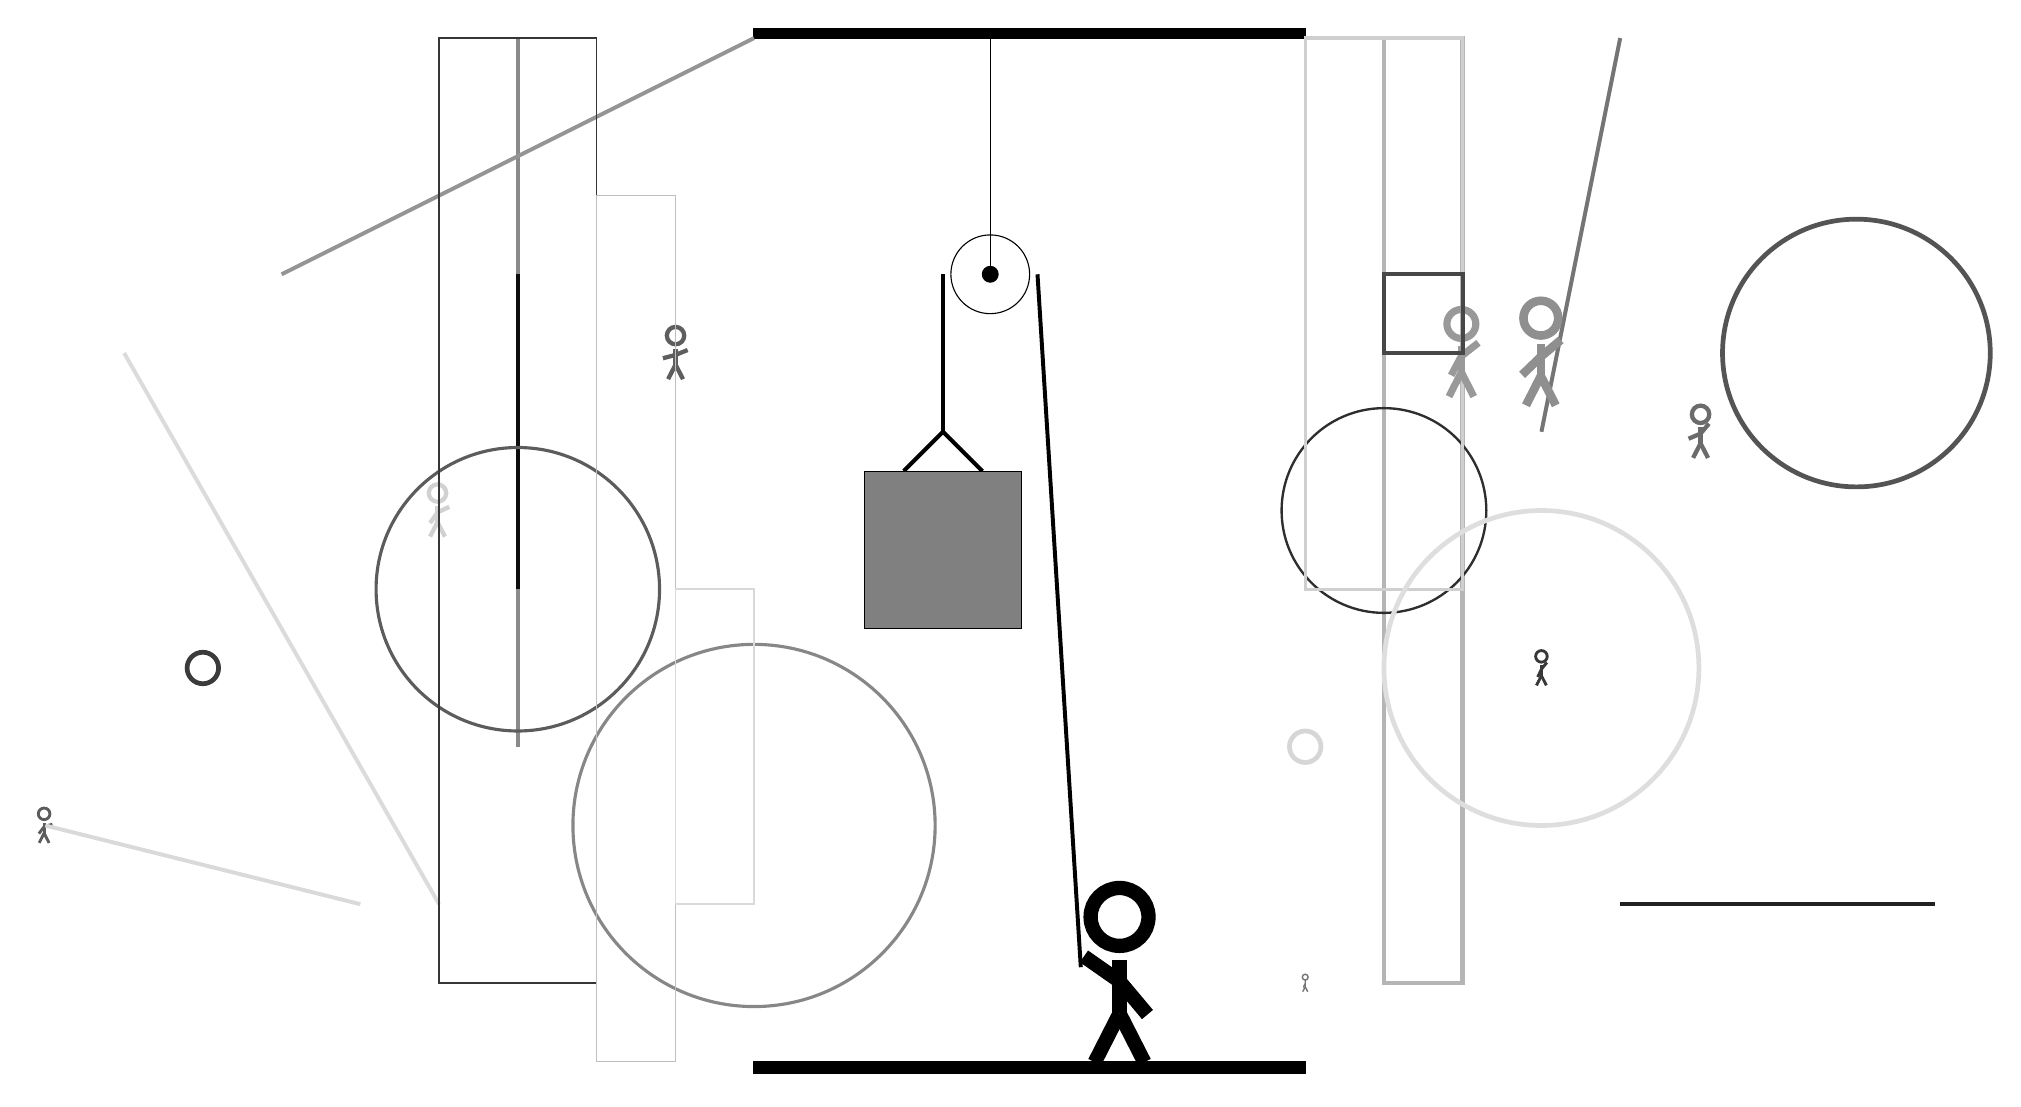
\begin{tikzpicture}
		%%%%% START %%%%%
		
		\draw[fill=black] (-2, 10) rectangle (5, 10.125);
		
		\draw (1, 7) circle (0.5);
		\draw[fill=black] (1, 7) circle (0.1);
		\draw (1, 10) -- (1, 7);
		
		\draw[line width=0.5mm] (-0.1, 4.5) -- (0.4, 5.0) -- (0.9, 4.5);
		\draw[fill=black!50] (-0.6, 4.5) rectangle (1.4, 2.5);
		
		\draw[line width=0.5mm] (0.4, 7) -- (0.4, 5.0);
		\centerarc[line width=0.5mm](1, 7)(0:180:0.6);
		\draw[line width=0.5mm](1.6, 7) -- (2.15, -1.8);
		
		\draw[line width=0.6mm, color=black!29] (6, -2) rectangle (7, 10);
		
		\node[line width=0.7mm, color=black!64] at (-11, 0) {\Strichmaxerl[2][53][17]};
		\node[line width=0.3mm, color=black!18] at (-6, 4) {\Strichmaxerl[3][55][25]};
		\draw[line width=0.5mm, color=black!46](-5, 10) -- (-5, 1);
		
		\draw[line width=0.5mm, color=black!15](-7, -1) -- (-11, 0);
		\draw[line width=0.5mm, color=black!14](-6, -1) -- (-10, 6);
		\draw[line width=0.5mm, color=black!42](-2, 10) -- (-8, 7);
		\draw [line width=0.6mm, color=black!67](12, 6) circle (1.7);
		\draw[line width=0.5mm, color=black!95](-5, 7) -- (-5, 3);
		\node[line width=0.4mm, color=black!78] at (8, 2) {\Strichmaxerl[2][64][51]};
		\draw[line width=0.5mm, color=black!54](9, 10) -- (8, 5);
		\node[line width=0.7mm, color=black!63] at (-3, 6) {\Strichmaxerl[3][15][22]};
		\draw [line width=0.4mm, color=black!64](-5, 3) circle (1.8);
		\node[line width=0.6mm, color=black!54] at (5, -2) {\Strichmaxerl[1][64][88]};
		\draw [line width=0.3mm, color=black!82](6, 4) circle (1.3);
		\node[line width=0.3mm, color=black!58] at (10, 5) {\Strichmaxerl[3][23][50]};
		
		\draw[line width=0.2mm, color=black!79] (-4, 10) rectangle (-6, -2);
		
		\draw [line width=0.4mm, color=black!47](-2, 0) circle (2.3);
		\draw[line width=0.2mm, color=black!25] (-3, -3) rectangle (-4, 8);
		\draw [line width=0.6mm, color=black!16](5, 1) circle (0.2);
		\draw[line width=0.2mm, color=black!15] (-3, 3) rectangle (-2, -1);
		\draw[line width=0.4mm, color=black!19] (5, 3) rectangle (7, 10);
		
		\node[line width=0.6mm, color=black!40] at (7, 6) {\Strichmaxerl[5][62][38]};
		\draw [line width=0.6mm, color=black!13](8, 2) circle (2.0);
		\draw[line width=0.5mm, color=black!72] (7, 6) rectangle (6, 7);
		\draw[line width=0.5mm, color=black!87](9, -1) -- (13, -1);
		\draw [line width=0.6mm, color=black!77](-9, 2) circle (0.2);
		\node[line width=0.5mm, color=black!44] at (8, 6) {\Strichmaxerl[6][44][40]};
		
		
		\node at (2.6, -1.9) {\Strichmaxerl[10][-35][-50]};
		
		\draw[fill=black] (-2, -3) rectangle (5, -3.15);
		
		%%%%% END %%%%%
	\end{tikzpicture}
\end{document}